\documentclass[twoside]{book}

% Packages required by doxygen
\usepackage{fixltx2e}
\usepackage{calc}
\usepackage{doxygen}
\usepackage{graphicx}
\usepackage[utf8]{inputenc}
\usepackage{makeidx}
\usepackage{multicol}
\usepackage{multirow}
\PassOptionsToPackage{warn}{textcomp}
\usepackage{textcomp}
\usepackage[nointegrals]{wasysym}
\usepackage[table]{xcolor}

% NLS support packages
\usepackage[italian]{babel}

% Font selection
\usepackage[T1]{fontenc}
\usepackage{mathptmx}
\usepackage[scaled=.90]{helvet}
\usepackage{courier}
\usepackage{amssymb}
\usepackage{sectsty}
\renewcommand{\familydefault}{\sfdefault}
\allsectionsfont{%
  \fontseries{bc}\selectfont%
  \color{darkgray}%
}
\renewcommand{\DoxyLabelFont}{%
  \fontseries{bc}\selectfont%
  \color{darkgray}%
}
\newcommand{\+}{\discretionary{\mbox{\scriptsize$\hookleftarrow$}}{}{}}

% Page & text layout
\usepackage{geometry}
\geometry{%
  a4paper,%
  top=2.5cm,%
  bottom=2.5cm,%
  left=2.5cm,%
  right=2.5cm%
}
\tolerance=750
\hfuzz=15pt
\hbadness=750
\setlength{\emergencystretch}{15pt}
\setlength{\parindent}{0cm}
\setlength{\parskip}{0.2cm}
\makeatletter
\renewcommand{\paragraph}{%
  \@startsection{paragraph}{4}{0ex}{-1.0ex}{1.0ex}{%
    \normalfont\normalsize\bfseries\SS@parafont%
  }%
}
\renewcommand{\subparagraph}{%
  \@startsection{subparagraph}{5}{0ex}{-1.0ex}{1.0ex}{%
    \normalfont\normalsize\bfseries\SS@subparafont%
  }%
}
\makeatother

% Headers & footers
\usepackage{fancyhdr}
\pagestyle{fancyplain}
\fancyhead[LE]{\fancyplain{}{\bfseries\thepage}}
\fancyhead[CE]{\fancyplain{}{}}
\fancyhead[RE]{\fancyplain{}{\bfseries\leftmark}}
\fancyhead[LO]{\fancyplain{}{\bfseries\rightmark}}
\fancyhead[CO]{\fancyplain{}{}}
\fancyhead[RO]{\fancyplain{}{\bfseries\thepage}}
\fancyfoot[LE]{\fancyplain{}{}}
\fancyfoot[CE]{\fancyplain{}{}}
\fancyfoot[RE]{\fancyplain{}{\bfseries\scriptsize Generato Mar 16 Mag 2017 14\+:06\+:12 per Zynq-\/7000 Driver Pack da Doxygen }}
\fancyfoot[LO]{\fancyplain{}{\bfseries\scriptsize Generato Mar 16 Mag 2017 14\+:06\+:12 per Zynq-\/7000 Driver Pack da Doxygen }}
\fancyfoot[CO]{\fancyplain{}{}}
\fancyfoot[RO]{\fancyplain{}{}}
\renewcommand{\footrulewidth}{0.4pt}
\renewcommand{\chaptermark}[1]{%
  \markboth{#1}{}%
}
\renewcommand{\sectionmark}[1]{%
  \markright{\thesection\ #1}%
}

% Indices & bibliography
\usepackage{natbib}
\usepackage[titles]{tocloft}
\setcounter{tocdepth}{3}
\setcounter{secnumdepth}{5}
\makeindex

% Hyperlinks (required, but should be loaded last)
\usepackage{ifpdf}
\ifpdf
  \usepackage[pdftex,pagebackref=true]{hyperref}
\else
  \usepackage[ps2pdf,pagebackref=true]{hyperref}
\fi
\hypersetup{%
  colorlinks=true,%
  linkcolor=blue,%
  citecolor=blue,%
  unicode%
}

% Custom commands
\newcommand{\clearemptydoublepage}{%
  \newpage{\pagestyle{empty}\cleardoublepage}%
}


%===== C O N T E N T S =====

\begin{document}

% Titlepage & ToC
\hypersetup{pageanchor=false,
             bookmarks=true,
             bookmarksnumbered=true,
             pdfencoding=unicode
            }
\pagenumbering{roman}
\begin{titlepage}
\vspace*{7cm}
\begin{center}%
{\Large Zynq-\/7000 Driver Pack }\\
\vspace*{1cm}
{\large Generato da Doxygen 1.8.8}\\
\vspace*{0.5cm}
{\small Mar 16 Mag 2017 14:06:12}\\
\end{center}
\end{titlepage}
\clearemptydoublepage
\tableofcontents
\clearemptydoublepage
\pagenumbering{arabic}
\hypersetup{pageanchor=true}

%--- Begin generated contents ---
\chapter{Indice delle strutture dati}
\section{Strutture dati}
Queste sono le strutture dati con una loro breve descrizione\+:\begin{DoxyCompactList}
\item\contentsline{section}{\hyperlink{struct_g_p_i_o__t}{G\+P\+I\+O\+\_\+t} \\*Struttura che astrae un device G\+P\+I\+O }{\pageref{struct_g_p_i_o__t}}{}
\item\contentsline{section}{\hyperlink{struct_h_d44780___l_c_d__t}{H\+D44780\+\_\+\+L\+C\+D\+\_\+t} \\*Struttura opaca che astrae un device Display L\+C\+D con cntroller Hitachi H\+D44780, o compatibile. Un oggetto di tipo \hyperlink{struct_h_d44780___l_c_d__t}{H\+D44780\+\_\+\+L\+C\+D\+\_\+t} rappresenta un device lcd H\+D44780. Il modulo e' pensato per permettere la gestione di piu' display da parte dello stesso processore, agendo su oggetti \hyperlink{struct_h_d44780___l_c_d__t}{H\+D44780\+\_\+\+L\+C\+D\+\_\+t} diversi. Il modulo permette di utilizzare sia l'interfacciamento ad otto bit che quello a quattro bit, inizializzando il device opportunamente, attraverso l'uso delle funzioni H\+D44780\+\_\+\+Init8 e\+H\+D44780\+\_\+\+Init4. Il modulo fornisce anche semplici funzioni per la stampa di un carattere o di una stringa null-\/terminated di caratteri. Si veda la documentazione delle funzioni H\+D44780\+\_\+\+Printc e H\+D44780\+\_\+\+Print. Inoltre sono presenti diverse funzioni di utilita' generica, come quelle per la pulizia del display, per lo spostamento del cursore di un posto in avanti o indietro, alla riga in basso o in alto }{\pageref{struct_h_d44780___l_c_d__t}}{}
\item\contentsline{section}{\hyperlink{struct_zybo_button__t}{Zybo\+Button\+\_\+t} \\*Struttura opaca che astrae l'insieme dei button presenti sulla board Digilent Zybo; }{\pageref{struct_zybo_button__t}}{}
\item\contentsline{section}{\hyperlink{struct_zybo_led__t}{Zybo\+Led\+\_\+t} \\*Struttura opaca che astrae l'insieme dei Led presenti sulla board Digilent Zybo; }{\pageref{struct_zybo_led__t}}{}
\item\contentsline{section}{\hyperlink{struct_zybo_switch__t}{Zybo\+Switch\+\_\+t} \\*Struttura opaca che astrae l'insieme degli switch presenti sulla board Digilent Zybo; }{\pageref{struct_zybo_switch__t}}{}
\end{DoxyCompactList}

\chapter{Documentazione delle classi}
\hypertarget{struct_g_p_i_o__t}{\section{Riferimenti per la struct G\+P\+I\+O\+\_\+t}
\label{struct_g_p_i_o__t}\index{G\+P\+I\+O\+\_\+t@{G\+P\+I\+O\+\_\+t}}
}


Struttura che astrae un device G\+P\+I\+O.  




{\ttfamily \#include $<$gpio.\+h$>$}

\subsection*{Campi}
\begin{DoxyCompactItemize}
\item 
\hypertarget{struct_g_p_i_o__t_a79c591d5fa42efdf86abd98347fece90}{uint32\+\_\+t $\ast$ {\bfseries base\+\_\+address}}\label{struct_g_p_i_o__t_a79c591d5fa42efdf86abd98347fece90}

\item 
\hypertarget{struct_g_p_i_o__t_a09a2a45f731b02946ff6d3cd15c1a476}{uint8\+\_\+t {\bfseries width}}\label{struct_g_p_i_o__t_a09a2a45f731b02946ff6d3cd15c1a476}

\item 
\hypertarget{struct_g_p_i_o__t_a14886d03a6936e5edd25a9ad27af16bd}{uint8\+\_\+t {\bfseries enable\+\_\+offset}}\label{struct_g_p_i_o__t_a14886d03a6936e5edd25a9ad27af16bd}

\item 
\hypertarget{struct_g_p_i_o__t_abb65e5db6d4ad365a7c48d00e4af1f78}{uint8\+\_\+t {\bfseries write\+\_\+offset}}\label{struct_g_p_i_o__t_abb65e5db6d4ad365a7c48d00e4af1f78}

\item 
\hypertarget{struct_g_p_i_o__t_ab65acde67dc46f1d163e2ee468420b48}{uint8\+\_\+t {\bfseries read\+\_\+offset}}\label{struct_g_p_i_o__t_ab65acde67dc46f1d163e2ee468420b48}

\end{DoxyCompactItemize}


\subsection{Descrizione dettagliata}
Struttura che astrae un device G\+P\+I\+O. 

La documentazione per questa struct è stata generata a partire dal seguente file\+:\begin{DoxyCompactItemize}
\item 
G\+P\+I\+O/gpio.\+h\end{DoxyCompactItemize}

\hypertarget{struct_h_d44780___l_c_d__t}{\section{Riferimenti per la struct H\+D44780\+\_\+\+L\+C\+D\+\_\+t}
\label{struct_h_d44780___l_c_d__t}\index{H\+D44780\+\_\+\+L\+C\+D\+\_\+t@{H\+D44780\+\_\+\+L\+C\+D\+\_\+t}}
}


Struttura opaca che astrae un device Display L\+C\+D con cntroller Hitachi H\+D44780, o compatibile. Un oggetto di tipo \hyperlink{struct_h_d44780___l_c_d__t}{H\+D44780\+\_\+\+L\+C\+D\+\_\+t} rappresenta un device lcd H\+D44780. Il modulo e' pensato per permettere la gestione di piu' display da parte dello stesso processore, agendo su oggetti \hyperlink{struct_h_d44780___l_c_d__t}{H\+D44780\+\_\+\+L\+C\+D\+\_\+t} diversi. Il modulo permette di utilizzare sia l'interfacciamento ad otto bit che quello a quattro bit, inizializzando il device opportunamente, attraverso l'uso delle funzioni H\+D44780\+\_\+\+Init8 e\+H\+D44780\+\_\+\+Init4. Il modulo fornisce anche semplici funzioni per la stampa di un carattere o di una stringa null-\/terminated di caratteri. Si veda la documentazione delle funzioni H\+D44780\+\_\+\+Printc e H\+D44780\+\_\+\+Print. Inoltre sono presenti diverse funzioni di utilita' generica, come quelle per la pulizia del display, per lo spostamento del cursore di un posto in avanti o indietro, alla riga in basso o in alto.  




{\ttfamily \#include $<$hd44780.\+h$>$}

\subsection*{Campi}
\begin{DoxyCompactItemize}
\item 
G\+P\+I\+O\+\_\+t $\ast$ \hyperlink{struct_h_d44780___l_c_d__t_acb3116190992a4d8d26545c103304d27}{gpio}
\item 
G\+P\+I\+O\+\_\+mask \hyperlink{struct_h_d44780___l_c_d__t_a142ae0db638dca7ab42e2183a1311d32}{R\+S}
\item 
G\+P\+I\+O\+\_\+mask \hyperlink{struct_h_d44780___l_c_d__t_af8225e4a125a2159215dfa03372c305f}{R\+W}
\item 
G\+P\+I\+O\+\_\+mask \hyperlink{struct_h_d44780___l_c_d__t_a851ed1cefdadae2e5069d1364ae8fc9e}{E}
\item 
G\+P\+I\+O\+\_\+mask \hyperlink{struct_h_d44780___l_c_d__t_a7f1bd9ea66e1fa6d0667c3f60d2f155d}{Data7}
\item 
G\+P\+I\+O\+\_\+mask \hyperlink{struct_h_d44780___l_c_d__t_a6a787746d32e0e18dbd57202e547756b}{Data6}
\item 
G\+P\+I\+O\+\_\+mask \hyperlink{struct_h_d44780___l_c_d__t_aff5ae7b6e5cd6f96a13e719cd07e3f15}{Data5}
\item 
G\+P\+I\+O\+\_\+mask \hyperlink{struct_h_d44780___l_c_d__t_a923c685eba8920c56f33117410da2742}{Data4}
\item 
G\+P\+I\+O\+\_\+mask \hyperlink{struct_h_d44780___l_c_d__t_ae6f2e7b5a4aa8b82451e021f2f5b3a89}{Data3}
\item 
G\+P\+I\+O\+\_\+mask \hyperlink{struct_h_d44780___l_c_d__t_afb22274224118a94688f1809cda55501}{Data2}
\item 
G\+P\+I\+O\+\_\+mask \hyperlink{struct_h_d44780___l_c_d__t_a9b310a22b76c920feb015a3a3084b125}{Data1}
\item 
G\+P\+I\+O\+\_\+mask \hyperlink{struct_h_d44780___l_c_d__t_aed1ef3393be1a14aa7b2644585e5bb08}{Data0}
\item 
\hyperlink{group___h_d44780_gaaaea8b73e24f7658da4118f6b01b45f0}{H\+D44780\+\_\+\+Interface\+Mode\+\_\+t} \hyperlink{struct_h_d44780___l_c_d__t_a7c5a51b8cc5de5ee2cf42b884bd1bc67}{iface\+\_\+mode}
\end{DoxyCompactItemize}


\subsection{Descrizione dettagliata}
Struttura opaca che astrae un device Display L\+C\+D con cntroller Hitachi H\+D44780, o compatibile. Un oggetto di tipo \hyperlink{struct_h_d44780___l_c_d__t}{H\+D44780\+\_\+\+L\+C\+D\+\_\+t} rappresenta un device lcd H\+D44780. Il modulo e' pensato per permettere la gestione di piu' display da parte dello stesso processore, agendo su oggetti \hyperlink{struct_h_d44780___l_c_d__t}{H\+D44780\+\_\+\+L\+C\+D\+\_\+t} diversi. Il modulo permette di utilizzare sia l'interfacciamento ad otto bit che quello a quattro bit, inizializzando il device opportunamente, attraverso l'uso delle funzioni H\+D44780\+\_\+\+Init8 e\+H\+D44780\+\_\+\+Init4. Il modulo fornisce anche semplici funzioni per la stampa di un carattere o di una stringa null-\/terminated di caratteri. Si veda la documentazione delle funzioni H\+D44780\+\_\+\+Printc e H\+D44780\+\_\+\+Print. Inoltre sono presenti diverse funzioni di utilita' generica, come quelle per la pulizia del display, per lo spostamento del cursore di un posto in avanti o indietro, alla riga in basso o in alto. 

\subsection{Documentazione dei campi}
\hypertarget{struct_h_d44780___l_c_d__t_aed1ef3393be1a14aa7b2644585e5bb08}{\index{H\+D44780\+\_\+\+L\+C\+D\+\_\+t@{H\+D44780\+\_\+\+L\+C\+D\+\_\+t}!Data0@{Data0}}
\index{Data0@{Data0}!H\+D44780\+\_\+\+L\+C\+D\+\_\+t@{H\+D44780\+\_\+\+L\+C\+D\+\_\+t}}
\subsubsection[{Data0}]{\setlength{\rightskip}{0pt plus 5cm}G\+P\+I\+O\+\_\+mask Data0}}\label{struct_h_d44780___l_c_d__t_aed1ef3393be1a14aa7b2644585e5bb08}
maschera di selezione per il pin del device G\+P\+I\+O usato per il pilotaggio del segnale D0 \hypertarget{struct_h_d44780___l_c_d__t_a9b310a22b76c920feb015a3a3084b125}{\index{H\+D44780\+\_\+\+L\+C\+D\+\_\+t@{H\+D44780\+\_\+\+L\+C\+D\+\_\+t}!Data1@{Data1}}
\index{Data1@{Data1}!H\+D44780\+\_\+\+L\+C\+D\+\_\+t@{H\+D44780\+\_\+\+L\+C\+D\+\_\+t}}
\subsubsection[{Data1}]{\setlength{\rightskip}{0pt plus 5cm}G\+P\+I\+O\+\_\+mask Data1}}\label{struct_h_d44780___l_c_d__t_a9b310a22b76c920feb015a3a3084b125}
maschera di selezione per il pin del device G\+P\+I\+O usato per il pilotaggio del segnale D1 \hypertarget{struct_h_d44780___l_c_d__t_afb22274224118a94688f1809cda55501}{\index{H\+D44780\+\_\+\+L\+C\+D\+\_\+t@{H\+D44780\+\_\+\+L\+C\+D\+\_\+t}!Data2@{Data2}}
\index{Data2@{Data2}!H\+D44780\+\_\+\+L\+C\+D\+\_\+t@{H\+D44780\+\_\+\+L\+C\+D\+\_\+t}}
\subsubsection[{Data2}]{\setlength{\rightskip}{0pt plus 5cm}G\+P\+I\+O\+\_\+mask Data2}}\label{struct_h_d44780___l_c_d__t_afb22274224118a94688f1809cda55501}
maschera di selezione per il pin del device G\+P\+I\+O usato per il pilotaggio del segnale D2 \hypertarget{struct_h_d44780___l_c_d__t_ae6f2e7b5a4aa8b82451e021f2f5b3a89}{\index{H\+D44780\+\_\+\+L\+C\+D\+\_\+t@{H\+D44780\+\_\+\+L\+C\+D\+\_\+t}!Data3@{Data3}}
\index{Data3@{Data3}!H\+D44780\+\_\+\+L\+C\+D\+\_\+t@{H\+D44780\+\_\+\+L\+C\+D\+\_\+t}}
\subsubsection[{Data3}]{\setlength{\rightskip}{0pt plus 5cm}G\+P\+I\+O\+\_\+mask Data3}}\label{struct_h_d44780___l_c_d__t_ae6f2e7b5a4aa8b82451e021f2f5b3a89}
maschera di selezione per il pin del device G\+P\+I\+O usato per il pilotaggio del segnale D3 \hypertarget{struct_h_d44780___l_c_d__t_a923c685eba8920c56f33117410da2742}{\index{H\+D44780\+\_\+\+L\+C\+D\+\_\+t@{H\+D44780\+\_\+\+L\+C\+D\+\_\+t}!Data4@{Data4}}
\index{Data4@{Data4}!H\+D44780\+\_\+\+L\+C\+D\+\_\+t@{H\+D44780\+\_\+\+L\+C\+D\+\_\+t}}
\subsubsection[{Data4}]{\setlength{\rightskip}{0pt plus 5cm}G\+P\+I\+O\+\_\+mask Data4}}\label{struct_h_d44780___l_c_d__t_a923c685eba8920c56f33117410da2742}
maschera di selezione per il pin del device G\+P\+I\+O usato per il pilotaggio del segnale D4 \hypertarget{struct_h_d44780___l_c_d__t_aff5ae7b6e5cd6f96a13e719cd07e3f15}{\index{H\+D44780\+\_\+\+L\+C\+D\+\_\+t@{H\+D44780\+\_\+\+L\+C\+D\+\_\+t}!Data5@{Data5}}
\index{Data5@{Data5}!H\+D44780\+\_\+\+L\+C\+D\+\_\+t@{H\+D44780\+\_\+\+L\+C\+D\+\_\+t}}
\subsubsection[{Data5}]{\setlength{\rightskip}{0pt plus 5cm}G\+P\+I\+O\+\_\+mask Data5}}\label{struct_h_d44780___l_c_d__t_aff5ae7b6e5cd6f96a13e719cd07e3f15}
maschera di selezione per il pin del device G\+P\+I\+O usato per il pilotaggio del segnale D5 \hypertarget{struct_h_d44780___l_c_d__t_a6a787746d32e0e18dbd57202e547756b}{\index{H\+D44780\+\_\+\+L\+C\+D\+\_\+t@{H\+D44780\+\_\+\+L\+C\+D\+\_\+t}!Data6@{Data6}}
\index{Data6@{Data6}!H\+D44780\+\_\+\+L\+C\+D\+\_\+t@{H\+D44780\+\_\+\+L\+C\+D\+\_\+t}}
\subsubsection[{Data6}]{\setlength{\rightskip}{0pt plus 5cm}G\+P\+I\+O\+\_\+mask Data6}}\label{struct_h_d44780___l_c_d__t_a6a787746d32e0e18dbd57202e547756b}
maschera di selezione per il pin del device G\+P\+I\+O usato per il pilotaggio del segnale D6 \hypertarget{struct_h_d44780___l_c_d__t_a7f1bd9ea66e1fa6d0667c3f60d2f155d}{\index{H\+D44780\+\_\+\+L\+C\+D\+\_\+t@{H\+D44780\+\_\+\+L\+C\+D\+\_\+t}!Data7@{Data7}}
\index{Data7@{Data7}!H\+D44780\+\_\+\+L\+C\+D\+\_\+t@{H\+D44780\+\_\+\+L\+C\+D\+\_\+t}}
\subsubsection[{Data7}]{\setlength{\rightskip}{0pt plus 5cm}G\+P\+I\+O\+\_\+mask Data7}}\label{struct_h_d44780___l_c_d__t_a7f1bd9ea66e1fa6d0667c3f60d2f155d}
maschera di selezione per il pin del device G\+P\+I\+O usato per il pilotaggio del segnale D7 \hypertarget{struct_h_d44780___l_c_d__t_a851ed1cefdadae2e5069d1364ae8fc9e}{\index{H\+D44780\+\_\+\+L\+C\+D\+\_\+t@{H\+D44780\+\_\+\+L\+C\+D\+\_\+t}!E@{E}}
\index{E@{E}!H\+D44780\+\_\+\+L\+C\+D\+\_\+t@{H\+D44780\+\_\+\+L\+C\+D\+\_\+t}}
\subsubsection[{E}]{\setlength{\rightskip}{0pt plus 5cm}G\+P\+I\+O\+\_\+mask E}}\label{struct_h_d44780___l_c_d__t_a851ed1cefdadae2e5069d1364ae8fc9e}
maschera di selezione per il pin del device G\+P\+I\+O usato per il pilotaggio del segnale E \hypertarget{struct_h_d44780___l_c_d__t_acb3116190992a4d8d26545c103304d27}{\index{H\+D44780\+\_\+\+L\+C\+D\+\_\+t@{H\+D44780\+\_\+\+L\+C\+D\+\_\+t}!gpio@{gpio}}
\index{gpio@{gpio}!H\+D44780\+\_\+\+L\+C\+D\+\_\+t@{H\+D44780\+\_\+\+L\+C\+D\+\_\+t}}
\subsubsection[{gpio}]{\setlength{\rightskip}{0pt plus 5cm}G\+P\+I\+O\+\_\+t$\ast$ gpio}}\label{struct_h_d44780___l_c_d__t_acb3116190992a4d8d26545c103304d27}
puntatore a struttura G\+P\+I\+O\+\_\+t, che astrae il particolare G\+P\+I\+O usato per il pilotaggio del display \hypertarget{struct_h_d44780___l_c_d__t_a7c5a51b8cc5de5ee2cf42b884bd1bc67}{\index{H\+D44780\+\_\+\+L\+C\+D\+\_\+t@{H\+D44780\+\_\+\+L\+C\+D\+\_\+t}!iface\+\_\+mode@{iface\+\_\+mode}}
\index{iface\+\_\+mode@{iface\+\_\+mode}!H\+D44780\+\_\+\+L\+C\+D\+\_\+t@{H\+D44780\+\_\+\+L\+C\+D\+\_\+t}}
\subsubsection[{iface\+\_\+mode}]{\setlength{\rightskip}{0pt plus 5cm}{\bf H\+D44780\+\_\+\+Interface\+Mode\+\_\+t} iface\+\_\+mode}}\label{struct_h_d44780___l_c_d__t_a7c5a51b8cc5de5ee2cf42b884bd1bc67}
modalita' di funzionamento dell'interfaccia verso il displau (4 oppure 8 bit) \hypertarget{struct_h_d44780___l_c_d__t_a142ae0db638dca7ab42e2183a1311d32}{\index{H\+D44780\+\_\+\+L\+C\+D\+\_\+t@{H\+D44780\+\_\+\+L\+C\+D\+\_\+t}!R\+S@{R\+S}}
\index{R\+S@{R\+S}!H\+D44780\+\_\+\+L\+C\+D\+\_\+t@{H\+D44780\+\_\+\+L\+C\+D\+\_\+t}}
\subsubsection[{R\+S}]{\setlength{\rightskip}{0pt plus 5cm}G\+P\+I\+O\+\_\+mask R\+S}}\label{struct_h_d44780___l_c_d__t_a142ae0db638dca7ab42e2183a1311d32}
maschera di selezione per il pin del device G\+P\+I\+O usato per il pilotaggio del segnale R\+S \hypertarget{struct_h_d44780___l_c_d__t_af8225e4a125a2159215dfa03372c305f}{\index{H\+D44780\+\_\+\+L\+C\+D\+\_\+t@{H\+D44780\+\_\+\+L\+C\+D\+\_\+t}!R\+W@{R\+W}}
\index{R\+W@{R\+W}!H\+D44780\+\_\+\+L\+C\+D\+\_\+t@{H\+D44780\+\_\+\+L\+C\+D\+\_\+t}}
\subsubsection[{R\+W}]{\setlength{\rightskip}{0pt plus 5cm}G\+P\+I\+O\+\_\+mask R\+W}}\label{struct_h_d44780___l_c_d__t_af8225e4a125a2159215dfa03372c305f}
maschera di selezione per il pin del device G\+P\+I\+O usato per il pilotaggio del segnale R\+W 

La documentazione per questa struct è stata generata a partire dal seguente file\+:\begin{DoxyCompactItemize}
\item 
Lcd/\hyperlink{hd44780_8h}{hd44780.\+h}\end{DoxyCompactItemize}

\hypertarget{struct_zybo_button__t}{\section{Riferimenti per la struct Zybo\+Button\+\_\+t}
\label{struct_zybo_button__t}\index{Zybo\+Button\+\_\+t@{Zybo\+Button\+\_\+t}}
}


Struttura opaca che astrae l'insieme dei button presenti sulla board Digilent Zybo;.  




{\ttfamily \#include $<$Zybo\+Button.\+h$>$}



Diagramma di collaborazione per Zybo\+Button\+\_\+t\+:\nopagebreak
\begin{figure}[H]
\begin{center}
\leavevmode
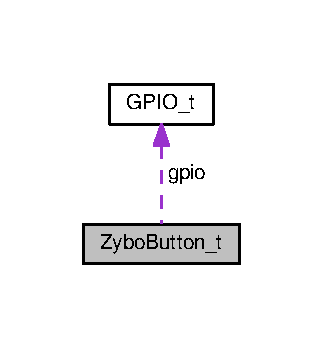
\includegraphics[width=155pt]{struct_zybo_button__t__coll__graph}
\end{center}
\end{figure}
\subsection*{Campi}
\begin{DoxyCompactItemize}
\item 
\hyperlink{structmy_g_p_i_o__t}{my\+G\+P\+I\+O\+\_\+t} $\ast$ \hyperlink{struct_zybo_button__t_ac37ddc7c58d246d233dfb38037020184}{gpio}
\item 
\hyperlink{group__bare-metal_ga402a0d20afc0cb7c25554b8b023f4253}{my\+G\+P\+I\+O\+\_\+mask} \hyperlink{struct_zybo_button__t_ad462a15a55883fd4c86d2be9e11968a7}{Button3\+\_\+pin}
\item 
\hyperlink{group__bare-metal_ga402a0d20afc0cb7c25554b8b023f4253}{my\+G\+P\+I\+O\+\_\+mask} \hyperlink{struct_zybo_button__t_a3b4fe634c2d98ce55fdef526c2d230d1}{Button2\+\_\+pin}
\item 
\hyperlink{group__bare-metal_ga402a0d20afc0cb7c25554b8b023f4253}{my\+G\+P\+I\+O\+\_\+mask} \hyperlink{struct_zybo_button__t_a6cb60bb285e32e29c51c15e85206aaeb}{Button1\+\_\+pin}
\item 
\hyperlink{group__bare-metal_ga402a0d20afc0cb7c25554b8b023f4253}{my\+G\+P\+I\+O\+\_\+mask} \hyperlink{struct_zybo_button__t_af7d7d5a9c9fc174e8f4ee4c762c2abee}{Button0\+\_\+pin}
\end{DoxyCompactItemize}


\subsection{Descrizione dettagliata}
Struttura opaca che astrae l'insieme dei button presenti sulla board Digilent Zybo;. \begin{Desc}
\item[Esempi\+: ]\par
\hyperlink{bsp_example_8c-example}{bsp\+\_\+example.\+c}.\end{Desc}


\subsection{Documentazione dei campi}
\hypertarget{struct_zybo_button__t_af7d7d5a9c9fc174e8f4ee4c762c2abee}{\index{Zybo\+Button\+\_\+t@{Zybo\+Button\+\_\+t}!Button0\+\_\+pin@{Button0\+\_\+pin}}
\index{Button0\+\_\+pin@{Button0\+\_\+pin}!Zybo\+Button\+\_\+t@{Zybo\+Button\+\_\+t}}
\subsubsection[{Button0\+\_\+pin}]{\setlength{\rightskip}{0pt plus 5cm}{\bf my\+G\+P\+I\+O\+\_\+mask} Button0\+\_\+pin}}\label{struct_zybo_button__t_af7d7d5a9c9fc174e8f4ee4c762c2abee}
maschera di selezione per il particolare bit del device my\+G\+P\+I\+O connesso al button numero 0 della board Zybo \hypertarget{struct_zybo_button__t_a6cb60bb285e32e29c51c15e85206aaeb}{\index{Zybo\+Button\+\_\+t@{Zybo\+Button\+\_\+t}!Button1\+\_\+pin@{Button1\+\_\+pin}}
\index{Button1\+\_\+pin@{Button1\+\_\+pin}!Zybo\+Button\+\_\+t@{Zybo\+Button\+\_\+t}}
\subsubsection[{Button1\+\_\+pin}]{\setlength{\rightskip}{0pt plus 5cm}{\bf my\+G\+P\+I\+O\+\_\+mask} Button1\+\_\+pin}}\label{struct_zybo_button__t_a6cb60bb285e32e29c51c15e85206aaeb}
maschera di selezione per il particolare bit del device my\+G\+P\+I\+O connesso al button numero 1 della board Zybo \hypertarget{struct_zybo_button__t_a3b4fe634c2d98ce55fdef526c2d230d1}{\index{Zybo\+Button\+\_\+t@{Zybo\+Button\+\_\+t}!Button2\+\_\+pin@{Button2\+\_\+pin}}
\index{Button2\+\_\+pin@{Button2\+\_\+pin}!Zybo\+Button\+\_\+t@{Zybo\+Button\+\_\+t}}
\subsubsection[{Button2\+\_\+pin}]{\setlength{\rightskip}{0pt plus 5cm}{\bf my\+G\+P\+I\+O\+\_\+mask} Button2\+\_\+pin}}\label{struct_zybo_button__t_a3b4fe634c2d98ce55fdef526c2d230d1}
maschera di selezione per il particolare bit del device my\+G\+P\+I\+O connesso al button numero 2 della board Zybo \hypertarget{struct_zybo_button__t_ad462a15a55883fd4c86d2be9e11968a7}{\index{Zybo\+Button\+\_\+t@{Zybo\+Button\+\_\+t}!Button3\+\_\+pin@{Button3\+\_\+pin}}
\index{Button3\+\_\+pin@{Button3\+\_\+pin}!Zybo\+Button\+\_\+t@{Zybo\+Button\+\_\+t}}
\subsubsection[{Button3\+\_\+pin}]{\setlength{\rightskip}{0pt plus 5cm}{\bf my\+G\+P\+I\+O\+\_\+mask} Button3\+\_\+pin}}\label{struct_zybo_button__t_ad462a15a55883fd4c86d2be9e11968a7}
maschera di selezione per il particolare bit del device my\+G\+P\+I\+O connesso al button numero 3 della board Zybo \hypertarget{struct_zybo_button__t_ac37ddc7c58d246d233dfb38037020184}{\index{Zybo\+Button\+\_\+t@{Zybo\+Button\+\_\+t}!gpio@{gpio}}
\index{gpio@{gpio}!Zybo\+Button\+\_\+t@{Zybo\+Button\+\_\+t}}
\subsubsection[{gpio}]{\setlength{\rightskip}{0pt plus 5cm}{\bf my\+G\+P\+I\+O\+\_\+t}$\ast$ gpio}}\label{struct_zybo_button__t_ac37ddc7c58d246d233dfb38037020184}
puntatore a struttura \hyperlink{structmy_g_p_i_o__t}{my\+G\+P\+I\+O\+\_\+t}, che astrae il particolare my\+G\+P\+I\+O usato per la lettura dello stato dei button presenti sulla board 

La documentazione per questa struct è stata generata a partire dal seguente file\+:\begin{DoxyCompactItemize}
\item 
Src/my\+G\+P\+I\+O/bare-\/metal/\+Zybo\+B\+S\+P/\hyperlink{_zybo_button_8h}{Zybo\+Button.\+h}\end{DoxyCompactItemize}

\hypertarget{struct_zybo_led__t}{\section{Riferimenti per la struct Zybo\+Led\+\_\+t}
\label{struct_zybo_led__t}\index{Zybo\+Led\+\_\+t@{Zybo\+Led\+\_\+t}}
}


Struttura opaca che astrae l'insieme dei Led presenti sulla board Digilent Zybo;.  




{\ttfamily \#include $<$Zybo\+Led.\+h$>$}



Diagramma di collaborazione per Zybo\+Led\+\_\+t\+:
\nopagebreak
\begin{figure}[H]
\begin{center}
\leavevmode
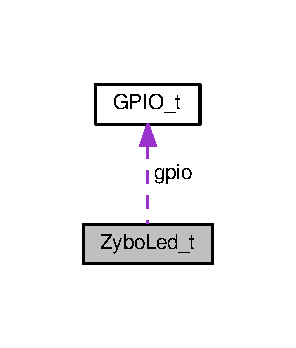
\includegraphics[width=143pt]{struct_zybo_led__t__coll__graph}
\end{center}
\end{figure}
\subsection*{Campi}
\begin{DoxyCompactItemize}
\item 
\hyperlink{structmy_g_p_i_o__t}{my\+G\+P\+I\+O\+\_\+t} $\ast$ \hyperlink{struct_zybo_led__t_ac37ddc7c58d246d233dfb38037020184}{gpio}
\item 
\hyperlink{group__my_g_p_i_o_ga402a0d20afc0cb7c25554b8b023f4253}{my\+G\+P\+I\+O\+\_\+mask} \hyperlink{struct_zybo_led__t_afc64d1407f30615e374bf9f06721842a}{Led3\+\_\+pin}
\item 
\hyperlink{group__my_g_p_i_o_ga402a0d20afc0cb7c25554b8b023f4253}{my\+G\+P\+I\+O\+\_\+mask} \hyperlink{struct_zybo_led__t_a4213c78e5a02b1476222e989c2eceb04}{Led2\+\_\+pin}
\item 
\hyperlink{group__my_g_p_i_o_ga402a0d20afc0cb7c25554b8b023f4253}{my\+G\+P\+I\+O\+\_\+mask} \hyperlink{struct_zybo_led__t_adc78fb167f1dd6693910813d4ec5930e}{Led1\+\_\+pin}
\item 
\hyperlink{group__my_g_p_i_o_ga402a0d20afc0cb7c25554b8b023f4253}{my\+G\+P\+I\+O\+\_\+mask} \hyperlink{struct_zybo_led__t_ac5afef2eef91d5533a23435cfcc60104}{Led0\+\_\+pin}
\end{DoxyCompactItemize}


\subsection{Descrizione dettagliata}
Struttura opaca che astrae l'insieme dei Led presenti sulla board Digilent Zybo;. 

\subsection{Documentazione dei campi}
\hypertarget{struct_zybo_led__t_ac37ddc7c58d246d233dfb38037020184}{\index{Zybo\+Led\+\_\+t@{Zybo\+Led\+\_\+t}!gpio@{gpio}}
\index{gpio@{gpio}!Zybo\+Led\+\_\+t@{Zybo\+Led\+\_\+t}}
\subsubsection[{gpio}]{\setlength{\rightskip}{0pt plus 5cm}{\bf my\+G\+P\+I\+O\+\_\+t}$\ast$ gpio}}\label{struct_zybo_led__t_ac37ddc7c58d246d233dfb38037020184}
puntatore a struttura \hyperlink{structmy_g_p_i_o__t}{my\+G\+P\+I\+O\+\_\+t}, che astrae il particolare G\+P\+I\+O usato per il pilotaggio dei led presenti sulla board \hypertarget{struct_zybo_led__t_ac5afef2eef91d5533a23435cfcc60104}{\index{Zybo\+Led\+\_\+t@{Zybo\+Led\+\_\+t}!Led0\+\_\+pin@{Led0\+\_\+pin}}
\index{Led0\+\_\+pin@{Led0\+\_\+pin}!Zybo\+Led\+\_\+t@{Zybo\+Led\+\_\+t}}
\subsubsection[{Led0\+\_\+pin}]{\setlength{\rightskip}{0pt plus 5cm}{\bf my\+G\+P\+I\+O\+\_\+mask} Led0\+\_\+pin}}\label{struct_zybo_led__t_ac5afef2eef91d5533a23435cfcc60104}
maschera di selezione per il particolare bit del device G\+P\+I\+O usato per il pilotaggio del led numero 0 della board Zybo \hypertarget{struct_zybo_led__t_adc78fb167f1dd6693910813d4ec5930e}{\index{Zybo\+Led\+\_\+t@{Zybo\+Led\+\_\+t}!Led1\+\_\+pin@{Led1\+\_\+pin}}
\index{Led1\+\_\+pin@{Led1\+\_\+pin}!Zybo\+Led\+\_\+t@{Zybo\+Led\+\_\+t}}
\subsubsection[{Led1\+\_\+pin}]{\setlength{\rightskip}{0pt plus 5cm}{\bf my\+G\+P\+I\+O\+\_\+mask} Led1\+\_\+pin}}\label{struct_zybo_led__t_adc78fb167f1dd6693910813d4ec5930e}
maschera di selezione per il particolare bit del device G\+P\+I\+O usato per il pilotaggio del led numero 1 della board Zybo \hypertarget{struct_zybo_led__t_a4213c78e5a02b1476222e989c2eceb04}{\index{Zybo\+Led\+\_\+t@{Zybo\+Led\+\_\+t}!Led2\+\_\+pin@{Led2\+\_\+pin}}
\index{Led2\+\_\+pin@{Led2\+\_\+pin}!Zybo\+Led\+\_\+t@{Zybo\+Led\+\_\+t}}
\subsubsection[{Led2\+\_\+pin}]{\setlength{\rightskip}{0pt plus 5cm}{\bf my\+G\+P\+I\+O\+\_\+mask} Led2\+\_\+pin}}\label{struct_zybo_led__t_a4213c78e5a02b1476222e989c2eceb04}
maschera di selezione per il particolare bit del device G\+P\+I\+O usato per il pilotaggio del led numero 2 della board Zybo \hypertarget{struct_zybo_led__t_afc64d1407f30615e374bf9f06721842a}{\index{Zybo\+Led\+\_\+t@{Zybo\+Led\+\_\+t}!Led3\+\_\+pin@{Led3\+\_\+pin}}
\index{Led3\+\_\+pin@{Led3\+\_\+pin}!Zybo\+Led\+\_\+t@{Zybo\+Led\+\_\+t}}
\subsubsection[{Led3\+\_\+pin}]{\setlength{\rightskip}{0pt plus 5cm}{\bf my\+G\+P\+I\+O\+\_\+mask} Led3\+\_\+pin}}\label{struct_zybo_led__t_afc64d1407f30615e374bf9f06721842a}
maschera di selezione per il particolare bit del device G\+P\+I\+O usato per il pilotaggio del led numero 3 della board Zybo 

La documentazione per questa struct è stata generata a partire dal seguente file\+:\begin{DoxyCompactItemize}
\item 
Zybo/\hyperlink{_zybo_led_8h}{Zybo\+Led.\+h}\end{DoxyCompactItemize}

\hypertarget{struct_zybo_switch__t}{\section{Riferimenti per la struct Zybo\+Switch\+\_\+t}
\label{struct_zybo_switch__t}\index{Zybo\+Switch\+\_\+t@{Zybo\+Switch\+\_\+t}}
}


Struttura opaca che astrae l'insieme degli switch presenti sulla board Digilent Zybo;.  




{\ttfamily \#include $<$Zybo\+Switch.\+h$>$}



Diagramma di collaborazione per Zybo\+Switch\+\_\+t\+:
\nopagebreak
\begin{figure}[H]
\begin{center}
\leavevmode
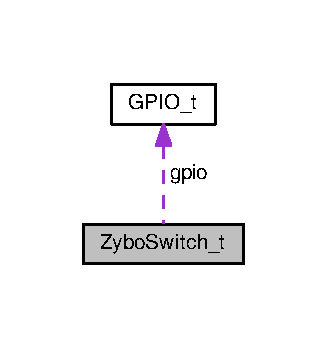
\includegraphics[width=157pt]{struct_zybo_switch__t__coll__graph}
\end{center}
\end{figure}
\subsection*{Campi}
\begin{DoxyCompactItemize}
\item 
\hypertarget{struct_zybo_switch__t_acb3116190992a4d8d26545c103304d27}{\hyperlink{struct_g_p_i_o__t}{G\+P\+I\+O\+\_\+t} $\ast$ {\bfseries gpio}}\label{struct_zybo_switch__t_acb3116190992a4d8d26545c103304d27}

\item 
\hypertarget{struct_zybo_switch__t_a6b95420b88fe8c1fd7f347ce3ae1906b}{G\+P\+I\+O\+\_\+mask {\bfseries Switch3\+\_\+pin}}\label{struct_zybo_switch__t_a6b95420b88fe8c1fd7f347ce3ae1906b}

\item 
\hypertarget{struct_zybo_switch__t_a33eda4a0115ef585edd90078924ca56e}{G\+P\+I\+O\+\_\+mask {\bfseries Switch2\+\_\+pin}}\label{struct_zybo_switch__t_a33eda4a0115ef585edd90078924ca56e}

\item 
\hypertarget{struct_zybo_switch__t_a6a3a5739e7e8f138241cafeeb7c1a33f}{G\+P\+I\+O\+\_\+mask {\bfseries Switch1\+\_\+pin}}\label{struct_zybo_switch__t_a6a3a5739e7e8f138241cafeeb7c1a33f}

\item 
\hypertarget{struct_zybo_switch__t_a5b7f83cd96441b7d1692710c6499147c}{G\+P\+I\+O\+\_\+mask {\bfseries Switch0\+\_\+pin}}\label{struct_zybo_switch__t_a5b7f83cd96441b7d1692710c6499147c}

\end{DoxyCompactItemize}


\subsection{Descrizione dettagliata}
Struttura opaca che astrae l'insieme degli switch presenti sulla board Digilent Zybo;. 

La documentazione per questa struct è stata generata a partire dal seguente file\+:\begin{DoxyCompactItemize}
\item 
Zybo/Zybo\+Switch.\+h\end{DoxyCompactItemize}

%--- End generated contents ---

% Index
\newpage
\phantomsection
\addcontentsline{toc}{chapter}{Indice}
\printindex

\end{document}
